\documentclass[12pt]{article}
\usepackage{amsmath}
\usepackage{amsfonts}
\usepackage{vmargin}
\usepackage[utf8]{inputenc}
\usepackage{graphicx}

\graphicspath{}

% \displaystyle is sooo important
\newcommand{\D}{\displaystyle}

\setmargins{2.5cm}
{0.1cm}
{16.5cm}
{23.42cm}
{10pt}
{1cm}
{0pt}
{2cm} 

\begin{document}
\title{
    \begin{figure}[ht]
        \centering
        
\includegraphics[width = 0.4\textwidth, ]{../../logo-uai.jpg}\\
    \end{figure}
    Ayudant\'ia \'Algebra Lineal N.3}
\date{26 de Agosto 2022}
\author{Daniel S\'anchez}
\maketitle

\begin{enumerate}
    \item Sean $A= \begin{bmatrix}
                  -1 & 0 & 2 \\
                  2  & 1 & 0
              \end{bmatrix}$ y $B=\begin{bmatrix}
                  -1 & 0 \\
                  1  & 2
              \end{bmatrix}$
          \begin{enumerate}
              \item Calcule $B\cdot A$
              \item Encuentre la matriz $X \in M_{2x2}(\mathbb{R})$ tal que:
                    $$A\cdot A^t+B\cdot X=(3I_2-2B)^t$$
          \end{enumerate}
          
          % OPCIONAL    
    \item Una empresa produce tres tipos de productos: $x_1, x_2 \mbox{ y }x_3$. La utilidad
          se obtiene mediante la siguiente relaci\'on:
          $$G(x_1,x_2,x_3)=20x_1-5x_2+10x_3$$
          y las cantidades a producir deben cumplir con las siguientes restricciones:
          $$\begin{array}{rcl}
                  x_1 - x_2 + 8x_3    & = & 50 \\
                  2x_1 + 3x_2 + 11x_3 & = & 60 \\
                  x_2 + 5x_3          & = & 30
              \end{array}$$
          \begin{enumerate}
              \item Resuelva el sistema, considerando que $x_1,x_2,x_3 \in \mathbb{{Z^+}_0}$
              \item Considere la soluci\'on en a) para obtener la utilidad.
          \end{enumerate}
          
    \item Determine el valor de verdad de:
          \begin{enumerate}
              \item Si $A \in M_{2x2}(\mathbb{R})$ es sim\'etrica y tiene inversa, entonces $A^{-1}$ tambi\'en es sim\'etrica.
              \item Si $A, B, C \in M_n(\mathbb{R})$ tal que $AB=AC$, entonces $B=C$.
          \end{enumerate}
          
    \item Utilice matrices por bloques para calcular la inversa de la siguiente matriz:
          $$\D A=\begin{bmatrix}
                  6 & -1/3 & 0  & 1    \\
                  3 & 0    & -1 & 0    \\
                  0 & 0    & 6  & -1/3 \\
                  0 & 0    & 3  & 0
              \end{bmatrix}$$
          \pagebreak
    \item El siguiente grafo representa rutas a\'ereas existentes entre varias ciudades y los costos, en
          d\'olares, de un pasaje en cada ruta. Todas las rutas pueden ser voladas de ida y de vuelta.
          \begin{figure}[ht]
              \centering
              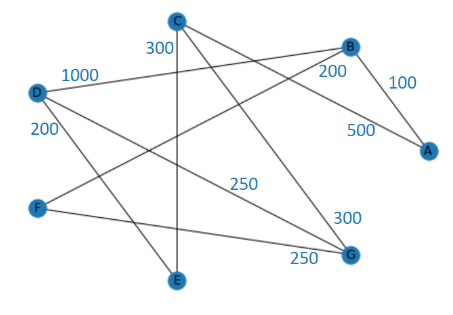
\includegraphics[width = 0.4\textwidth, ]{4.png}\\
          \end{figure}
          \begin{enumerate}
              \item Construya una matriz de adyacencia para el grafo dado.
              \item Encuentre la cantidad de rutas existentes entre cualquier par de ciudades que realicen
                    exactamente dos escalas intermedias.
              \item Considerando el costo total de los pasajes, determine cu\'al de las rutas entre las ciudades
                    A y D, que realizan exactamente dos escalas intermedias, es la m\'as econ\'omica.
          \end{enumerate}
\end{enumerate}
\end{document}